\chapter{\selectlanguage{greek}Θεωρητικό υπόβαθρο}
\begin{itemize}
\item περιγραφή πειράματος και
\item Για να καταλάβει ο κόσμος τι σημαίνει
\item Γιατί είναι χρήσιμο
\item Φωτογραφίες
\item Τι χρειάζεται να ξέρω
\item Το πείραμα
\end{itemize}

Στο κεφάλαιο αυτό παρουσιάζονται αναλυτικά οι 

\section{Το \en{CERN}}

To \en{CERN}, διατηρώντας το ακρωνύμιο της αρχικής Γαλλικής ονομασίας του \en{Conseil Européen pour la Recherche Nucléaire}, είναι το μεγαλύτερο σε έκταση πειραματικό κέντρο πυρηνικών ερευνών και ειδικότερα επί της σωματιδιακής φυσικής στον κόσμο. 
Βρίσκεται δυτικά της Γενεύης, στα σύνορα Ελβετίας και Γαλλίας. 
Ιδρύθηκε το 1954 από 12 ευρωπαϊκές χώρες και σήμερα αριθμεί 20 κράτη-μέλη, μεταξύ των οποίων και η Ελλάδα, η οποία είναι και ιδρυτικό μέλος.

\begin{figure}[h]

\includegraphics[scale=0.5]{images/LogoOutline-Black-01.png}
\centering
\caption{Το λογότυπο του \en{CERN}}
\label{CERNlogo}
\end{figure}

Η βασική λειτουργία του \en{CERN} είναι η παροχή επιταχυντών σωματιδίων και άλλων υποδομών απαραίτητων για την έρευνα στον τομέα της φυσικής υψηλών ενεργειών και ως αποτέλεσμα έχουν πραγματοποιηθεί πολυάριθμα πειράματα στο \en{CERN} μέσω διεθνών συνεργασιών.

Επίσης, το \en{CERN} αποτελεί τη γενέτειρα του Παγκόσμιου Ιστού (\en{World Wide Web}). Στην κύρια τοποθεσία του στο \en{Meyrin} βρίσκεται μεγάλη εγκατάσταση ηλεκτρονικών υπολογιστών με ισχυρές υποδομές επεξεργασίας δεδομένων, κυρίως για την ανάλυση των πειραματικών δεδομένων. 
Λόγω της ανάγκης να καταστούν αυτές διαθέσιμες σε εξωτερικούς ερευνητές, υπήρξε ιστορικά ένας σημαντικός κόμβος δικτύου ευρείας περιοχής (\en{Wide Area Network}).

Αρκετά σημαντικά επιτεύγματα στο πεδίο της φυσικής των σωματιδίων έγιναν μέσω πειραμάτων στο \en{CERN}. Αυτά περιλαμβάνουν:
\begin{itemize}
\item 1973: Ανακάλυψη των ουδέτερων ρευμάτων στο θάλαμο φυσαλίδων \en{Gargamelle}.
\item 1983: Ανακάλυψη των μποζονίων $W$ και $Z$ στα πειράματα \en{UA1} και \en{UA2}.
\item 1995: Πρώτη δημιουργία ατόμων αντιυδρογόνου στο πείραμα \en{PS210}.
\item 1999: Ανακάλυψη της άμεσης παραβίασης \en{CP} στο πείραμα \en{NA48}.
\item 2010: Απομόνωση 38 ατόμων αντιυδρογόνου.
\item 2011: Διατήρηση αντιυδρογόνου για πάνω από 15 λεπτά.
\item 2012: Ένα μποζόνιο με μάζα περίπου \SI[per-mode = symbol]{125}{\GeV \per  \clight \squared} συνάδει με τον πολυπόθητο μποζόνιο \en{Higgs}.
\end{itemize}


\section{Ο επιταχυντής \en{CLIC}}
\en{CLIC -- the Compact Linear Collider -- is a study for a future accelerator that will reach unprecedented energies for electrons and their antimatter twins, positrons. When they come into contact in the collision they will annihilate each other, liberating all their energy for the production of new particles.}

\en{Electrons and positrons are fundamental particles, and their collisions can provide extremely detailed information about the laws of nature. So CLIC would offer significant fundamental physics insight beyond that available from the Large Hadron Collider (LHC) and a lower-energy linear electron/positron collider, as a result of its unique combination of experimental precision and high energy.}

\en{At these high energies, electrons and positrons would lose a huge fraction of their energy circulating in a ring collider like the LHC. So the particles have to be accelerated in two linear accelerators facing each other, such that the beams collide in the central physics detector. This implies that the particles have to gain their energy in a single passage through the accelerating cavities.}

\begin{figure}[h]
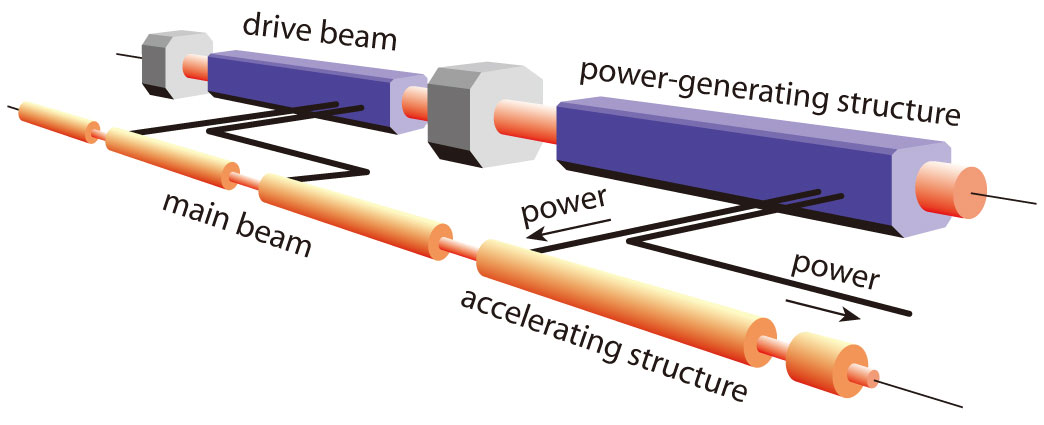
\includegraphics[width=0.5\textwidth]{images/CLIC-twobeam.jpg}
\centering
\caption{\en{CLIC two-beam scheme}}
\label{CLICtwobeamscheme}
\end{figure}

\en{CLIC is designed to be built in stages of increasing collision energy: starting from \SI{360}{\GeV}, around \SI{1.4}{\TeV}, and up to a final energy of \SI{3}{\TeV}. In order to reach this energy in a realistic and cost efficient scenario, the accelerating gradient has to be very high - CLIC aims at an acceleration of \SI[per-mode = symbol]{100}{\mega \volt \per \metre}, 20 times higher than the LHC.}

\en{This drive beam is decelerated in special Power Extraction and Transfer Structures (PETS), and the generated RF power is transferred to the main beam. This leads to a very simple tunnel layout without any active RF components (i.e. klystrons).}

\begin{figure}[h]
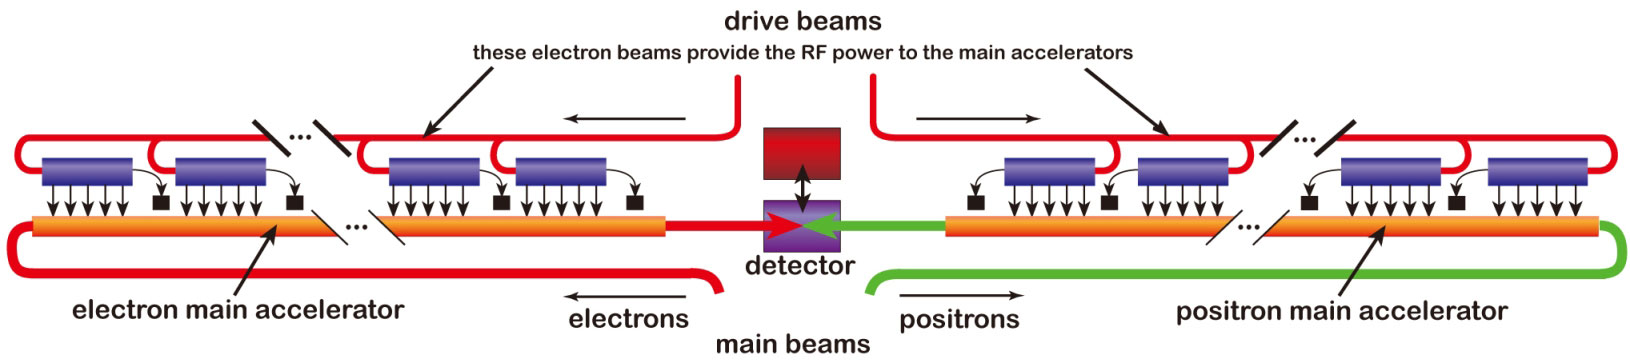
\includegraphics[width=\textwidth]{images/CLIC-layout.jpg}
\centering
\caption{\en{CLIC layout}}
\label{CLIClayout}
\end{figure}

\en{The feasibility of CLIC has been demonstrated and documented for the accelerator and the detector in the CLIC Conceptional Design Report. The design is currently being further optimized and adapted after the discovery of the Higgs boson at the LHC. CLIC is one of the options for a future accelerator built at CERN, which will be decided depending on future LHC physics results.}

\section{\en{Electron beam scanner}}

